\section*{Results}

\subsection*{One-dimensional optimization}
\begin{center}
    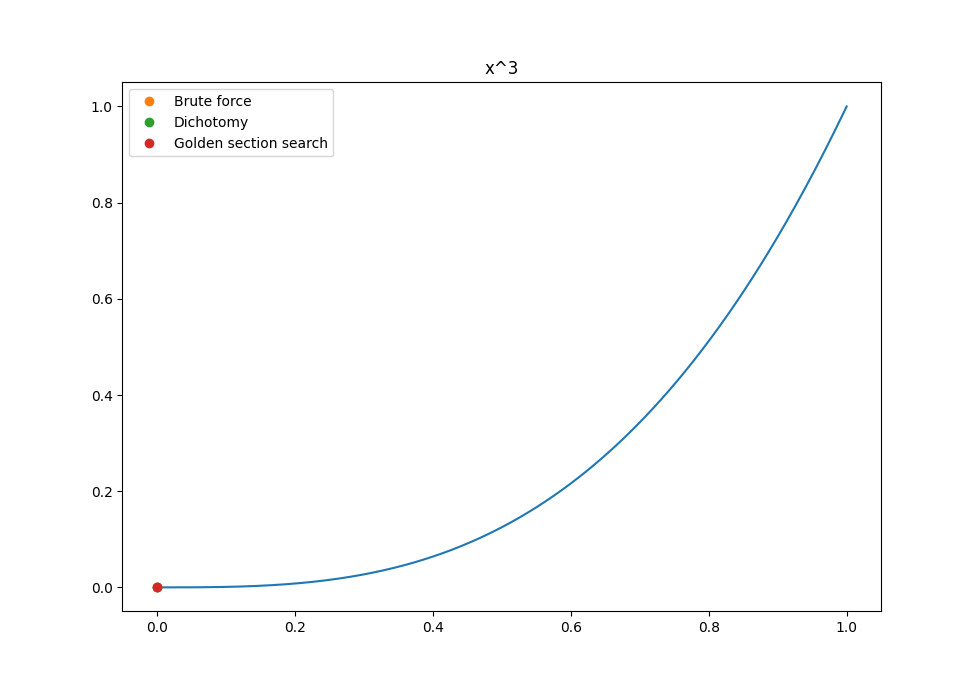
\includegraphics[width=0.7\textwidth]{../results/x_3.png}
    \captionof{figure}{$f(x) = x^3$ function minimization}
\end{center} 

\begin{table*}[h!]
    \begin{center}
        \caption{Optimization results on $f(x) = x^3$}
        \begin{tabular}{|c|c|c|c|c|}
            \textbf{Algorithm} & \textbf{$x$} & \textbf{$f(x)$} & \textbf{Evaluations} & \textbf{Iterations}\\
            \hline
            Real minimum & 0 & 0 & &\\
            Brute-force & 0.0005 & 1.25e-10 & 1000 & 1000 \\
            Dichotomy & 0.0003 & 2.38e-11 & 22 & 11 \\
            Golden-section search & 0.0004 & 4.93e-11 & 17 & 15
        \end{tabular}
    \end{center}
\end{table*}

\begin{center}
    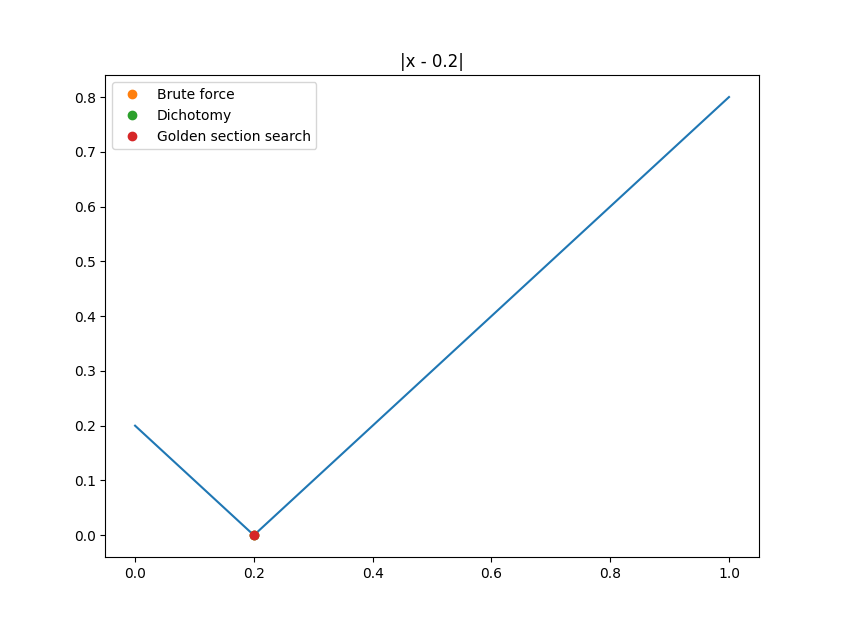
\includegraphics[width=0.7\textwidth]{../results/abs.png}
    \captionof{figure}{$f(x) = |x - 0.2|$ function minimization}
\end{center}

\begin{table*}[h!]
    \begin{center}
        \caption{Optimization results on $f(x) = |x - 0.2|$}
        \begin{tabular}{|c|c|c|c|c|}
            \textbf{Algorithm} & \textbf{$x$} & \textbf{$f(x)$} & \textbf{Evaluations} & \textbf{Iterations}\\
            \hline
            Real minimum & 0.2 & 0 & &\\
            Brute-force & 0.2005 & 0.0005 & 1000 & 1000 \\
            Dichotomy & 0.1999 & 2.27e-05 & 22 & 11 \\
            Golden-section search & 0.2001 & 7.33e-05 & 17 & 15
        \end{tabular}
    \end{center}
\end{table*}


\begin{center}
    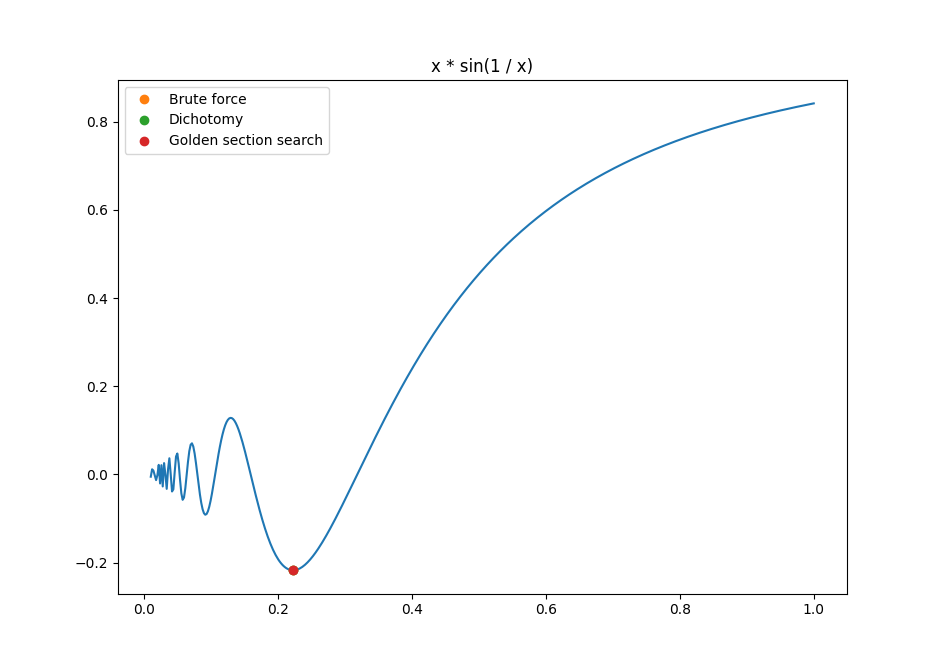
\includegraphics[width=0.7\textwidth]{../results/xsin.png}
    \captionof{figure}{$f(x) = x sin \frac{1}{x}$ function minimization}
\end{center}

\begin{table*}[h!]
    \begin{center}
        \caption{Optimization results on $f(x) = x sin\frac{1}{x}$}
        \begin{tabular}{|c|c|c|c|c|}
            \textbf{Algorithm} & \textbf{$x$} & \textbf{$f(x)$} & \textbf{Evaluations} & \textbf{Iterations}\\
            \hline
            Real minimum & 0.2225 & 0 & &\\
            Brute-force & 0.2235 & -0.2171 & 990 & 990 \\
            Dichotomy & 0.2225 & -0.2172 & 22 & 11 \\
            Golden-section search & 0.2227 & -0.2172 & 17 & 15
        \end{tabular}
    \end{center}
\end{table*}

For all functions the minimum point was found with given precision of $\epsilon = 0.001$. However, the last function does not meet requirements for
dichotomy and golden section methods (it is not convex on $[1;1]$), its form and initial bounds allows method to find minimum.

As it seen from results tables golden-section method is the most effective in terms of function evaluation counts. It require slightly more iterations then dichotomy method (its iteration count depends on delta value).
Brute-force method requires the most calculations.

\subsection*{Multidimensional optimization}

\begin{center}
    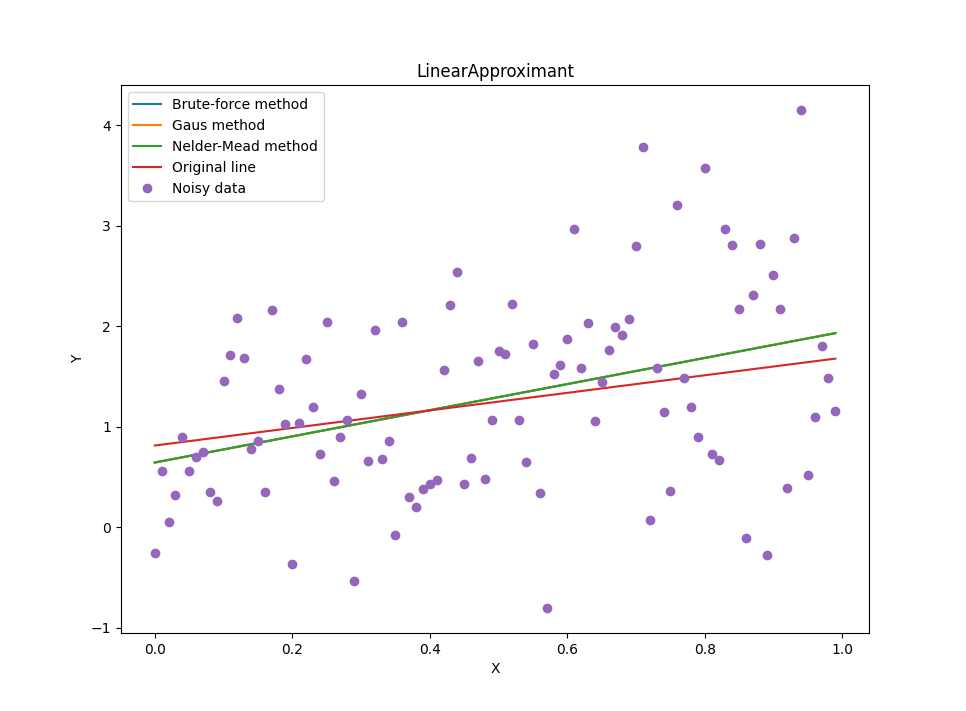
\includegraphics[width=0.7\textwidth]{../results/linear.png}
    \captionof{figure}{Linear approximant}
\end{center}

\begin{center}
    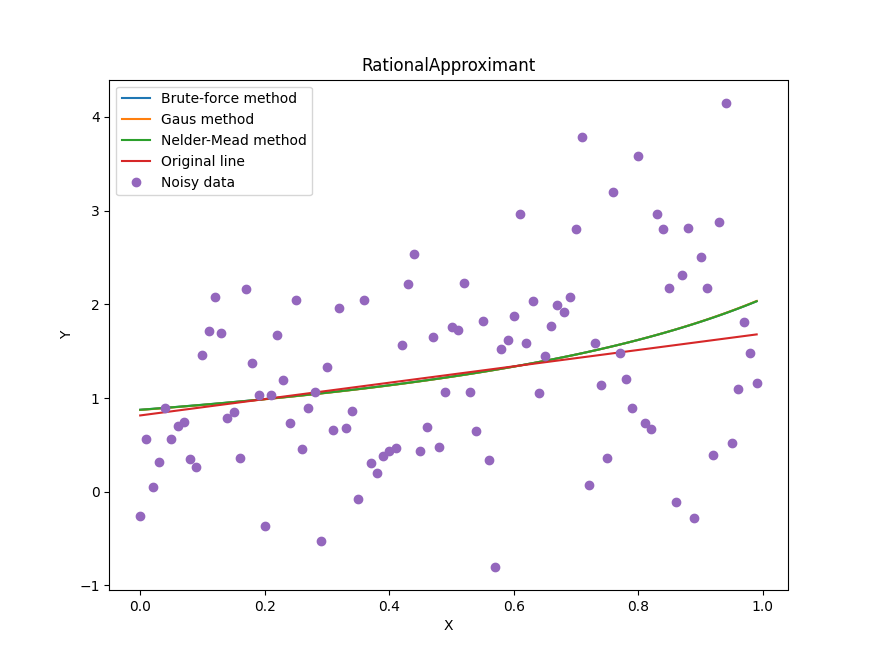
\includegraphics[width=0.7\textwidth]{../results/rational.png}
    \captionof{figure}{Rational approximant}
\end{center}

For both approximants all optimizers finds similar sollutions, although the particular found sollution depends 
on initial values (for Nelder-Mead method) and initial bounds (for brute-force and Gauss method).

\begin{table*}[h!]
    \begin{center}
        \caption{Optimization results on least squares method on bounds [0.0, 1.5], [0.0, 1.5]}
        \begin{tabular}{|c|c|c|c|c|}
            \textbf{Algorithm} & \textbf{$a, b$} & \textbf{$(\hat{y} - y)^2$} & \textbf{Evaluations} & \textbf{Iterations}\\
            \hline
            Real & (0.87, 0.81) & 82.36 & &\\
            Brute-force & (1.3004, 0.6455) & 80.6719 & 2253001 & 2253001 \\
            Gauss & (1.3028, 0.6434) & 80.6719 & 864 & 800 \\
            Nelder-Mead & (1.3000, 0.6448) & 80.6719 & 117 & 60
        \end{tabular}
    \end{center}
\end{table*}


Similarly to one-dimensional case the brute-force requires the most calculations. Nelder-Mead has the least count of function evaluations and iterations, although Gauss method (with use of golden-section method for one-dimensional optimization) has lower evaluations to iterations ratio.

